\documentclass[./main.tex]{subfiles}

\begin{document}
\begin{abstract}
\normalsize
Nella seguente analisi si vuole affrontare un problema di classificazione di attività motorie, utilizzando dati sull'accelerazione a cui è sottoposto un cellulare. Le attività devono essere classificate, con una particolare attenzione nell'identificare correttamente quando il cellulare viene agitato volontariamente ({\em shake}) o meno. Un campo applicativo per questo modello può essere un software per cellulare di monitoraggio di attività fisica, che integri delle funzionalità quando l'utente effettua uno {\em shake}. Classificare erroneamente un'attività come {\em shake} può essere fonte di disturbo per l'utente, se vengono attivate delle funzionalità quando non richiesto. Lo sviluppatore del software può essere interessato a minimizzare il disturbo arrecato all'utente, quindi a non classificare come {\em shake} attività diverse.
\end{abstract}
\section{Raccolta dei dati}
I dati sono stati raccolti sullo stesso cellulare, in campioni di circa $\SI{2}{\min}$ per attività, eseguita da persone diverse. La rilevazione dei dati è stata effettuata tramite l'applicazione \texttt{PhonePi}~\cite{kumar2019}.\\
Come attività motorie, è stato scelto il seguente insieme di attività quotidiane:
\begin{enumerate}
	\item Camminata con cellulare in mano.
	\item Camminata con cellulare in tasca.
	\item Corsa con cellulare in mano.
	\item Corsa con cellulare in tasca.
	\item Utilizzo a riposo (chiamate e scrittura di messaggi).
	\item Salti sul posto.
	\item Shake volontario.
\end{enumerate}
Per ciascuna classe, si dispongono di misurazioni a intervalli di ampiezza $\Delta t = \SI{10}{ms}$ della quantità
$$
\vec{a}_t = \begin{pmatrix}
a_{xt}\\
a_{yt}\\
a_{zt}
\end{pmatrix}\,,
$$
accelerazione del cellulare rispetto agli assi cartesiani di riferimento dell'accelerometro. L'analisi è stata condotta sull'intensità dell'accelerazione $a_t = \|\vec{a}_t\|$, ignorando l'effetto di disturbo dell'accelerazione di gravità. Da ogni campione sono stati tolti i primi e gli ultimi sette secondi, considerando solo i dati per le attività ``a regime''.
In Figura~\ref{fig:esempio} sono riportati dei grafici di esempio dei dati raccolti.
\begin{figure}[H]
	\label{fig:esempio}
	\centering
	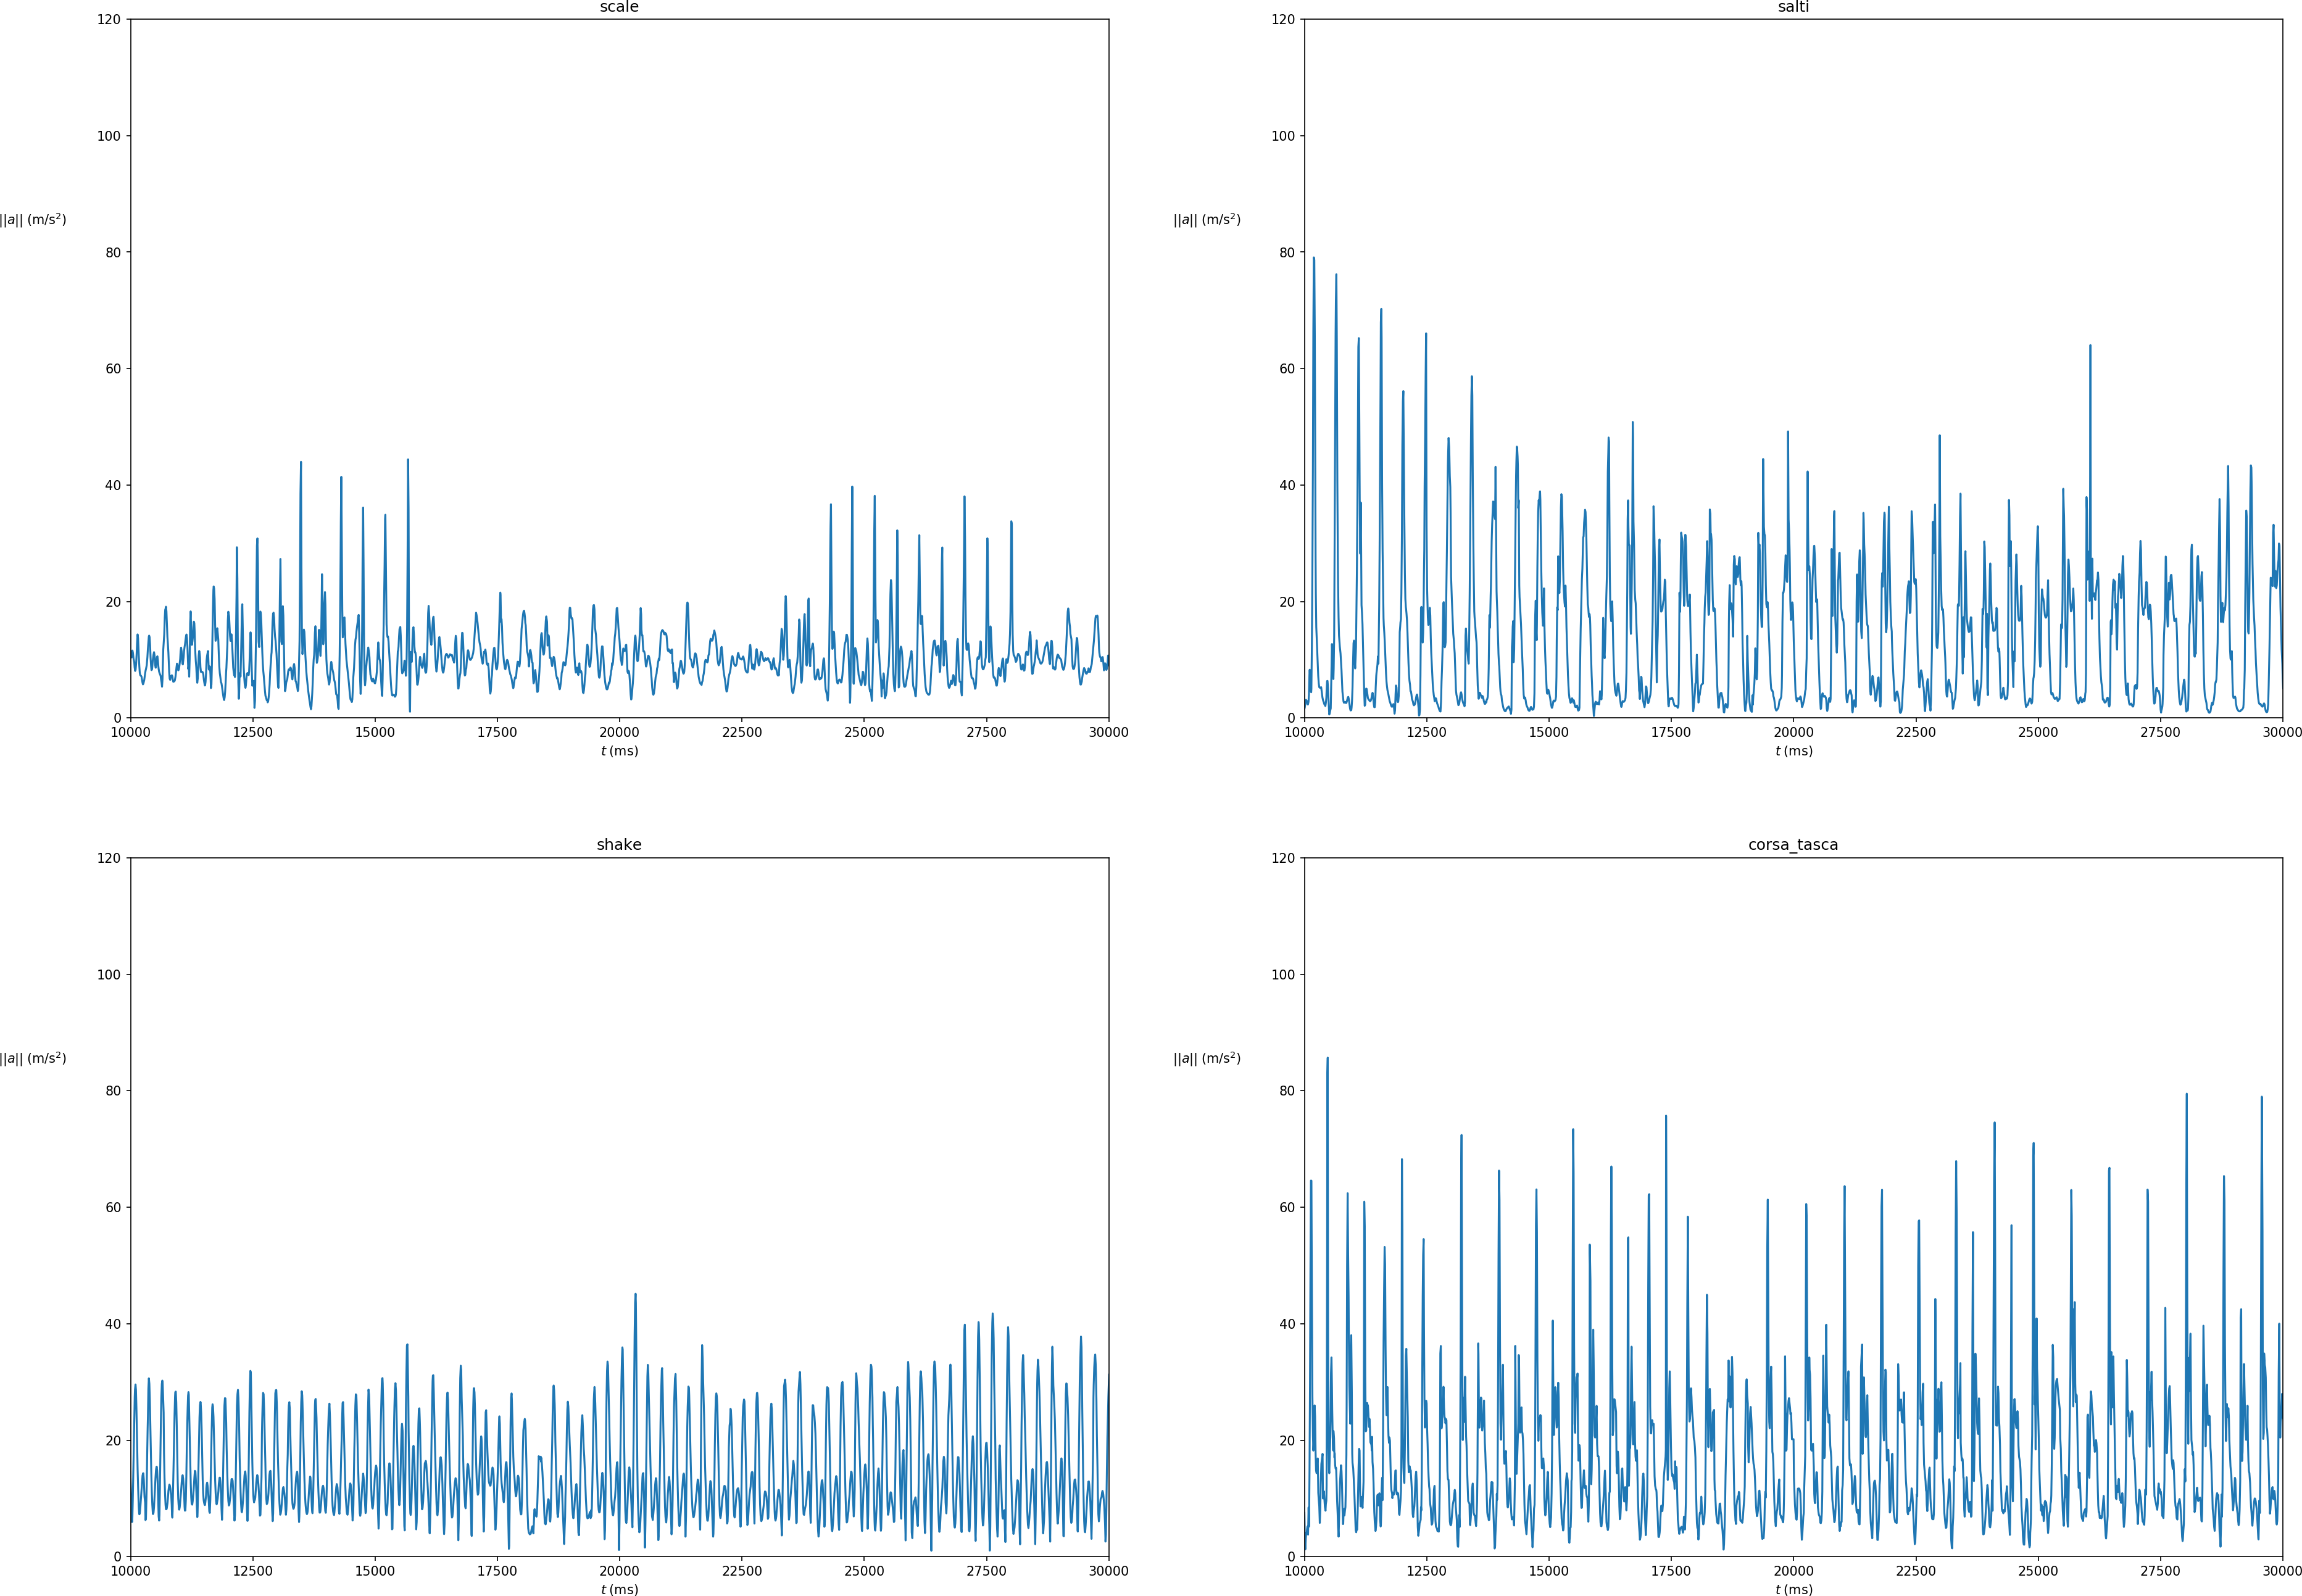
\includegraphics[width=.8\textwidth, keepaspectratio]{../../figure/espl.png}
	\caption{Intervalli $ [\SI{10}{\second}, \SI{30}{\second}] $ per le attività motorie di salita e discesa di scale, salti, shake, corsa con cellulare in tasca.}
\end{figure}
\end{document}